
%%%
%%% CHAPTER
%%%
\chapter{Thermodynamic Formulation}\label{Chapter:ThermodynamicFormulation}

%%%
%%% SECTION
%%%
\section{Mass Balance}\label{Chapter:ThermodynamicFormulation:Section:MassBalance}
Given a closed system at constant pressure and temperature conditions with $n_{c}$ components contained in $n_{p}$ phases. We can define a normalised concentration, \ie mole fraction $\left(\mfr[x]{i}{j}\right)$ based on the relationship between the number of moles of component $i$ at phase $j$ with the total number of moles contained in the same phase, 
\begin{equation}
    \mfr[x]{i}{j} = \frc{\mfr[n]{i}{j}}{\mfr[n]{}{j}} = \frc{\frc{\mfr[m]{i}{j}}{MW_{i}}}{\frc{\mfr[m]{}{j}}{\mfr[\overline{MW}]{}{j}}}, \hfill \text{ with } i=1, \cdots, n_{c} \text{ and } j=1, \cdots, n_{p}
\label{Chapter:ThermodynamicFormulation:Eqn:MoleFractionDef}
\end{equation}
where $MW$ is the molar mass, $n$ is the number of moles and $m$ is the mass. In this Chapter, superscripts and subscripts stand for phase and component identities, respectively.  For completeness, we can also define
\begin{eqnarray}
    z_{i} = \frc{n_{i}}{n} &=& \frc{\frc{m_{i}}{MW_{i}}}{\frc{m}{\overline{MW}}}\label{Chapter:ThermodynamicFormulation:Eqn:FeedFractionDef} \\
    \mfr[\Pi]{}{j} = \frc{\mfr[n]{}{j}}{n} &=& \frc{\frc{\mfr[m]{}{j}}{\mfr[\overline{MW}]{}{j}}}{\frc{m}{\overline{MW}}},\label{Chapter:ThermodynamicFormulation:Eqn:PhaseFractionDef} 
\end{eqnarray}
where $z_{i}$ is the overall feed molar fraction of component $i$, and $\Pi$ is the mole fraction of phase $j$. The relations above are subject to the following constraints:
\begin{equation}
    \summation_{i=1}^{n_{c}}\mfr[x]{i}{j} = 1 \;\;\;,\;\;\; \summation_{i=1}^{n_{c}}z_{i} = 1 \;\;\;,\;\;\; \summation_{j=1}^{n_{p}}\mfr[\Pi]{}{j} = 1. \label{Chapter:ThermodynamicFormulation:Eqn:FractionConstraints1}
\end{equation}
These linear constraints can be expressed as
\begin{equation}
    \mfr[x]{n_{c}}{j}= 1 - \summation_{i=1}^{n_{c}-1}\mfr[x]{i}{j} \;\;\;,\;\;\; z_{n_{c}}= 1 - \summation_{i=1}^{n_{c}-1}z_{i} \;\;\;,\;\;\; \mfr[\Pi]{}{n_{p}} = 1 - \summation_{j=1}^{n_{p}-1}\mfr[\Pi]{}{j} \label{Chapter:ThermodynamicFormulation:Eqn:FractionConstraints2}
\end{equation}
Equation~\ref{Chapter:ThermodynamicFormulation:Eqn:FeedFractionDef} can be rearranged as,
\begin{eqnarray}
  z_{i} &=& \frc{n_{i}}{n} = \frc{\summation_{j=1}^{n_{p}}\mfr[n]{i}{j}}{n} \cdot \frc{\summation_{j=1}^{n_{p}}\mfr[n]{}{j}}{\summation_{j=1}^{n_{p}}\mfr[n]{}{j}} = \underbrace{\frc{ \summation_{j=1}^{n_{p}}\mfr[n]{}{j}}{n}}_{\red{\summation_{j=1}^{n_{p}}\mfr[\Pi]{}{j}}} \cdot \overbrace{ \frc{\summation_{j=1}^{n_{p}}\mfr[n]{i}{j}}{\summation_{j=1}^{n_{p}}\mfr[n]{}{j}}}^{\red{\summation_{j=1}^{n_{p}}\mfr[x]{i}{j}}}, \nonumber \\
       &=& \summation_{j=1}^{n_{p}} \mfr[\Pi]{}{j}\mfr[x]{i}{j},\;\;\;\;\;i=1, \cdots, n_{c}\hfill\label{Chapter:ThermodynamicFormulation:Eqn:FeedFractionDef2} 
\end{eqnarray}
with 
\begin{equation}
      0\leq \mfr[x]{i}{j} \leq 1 \;\;\;\text{ and }\;\;\; 0\leq\mfr[\Pi]{}{j}\leq 1 \hfill
\end{equation}
If the solution is contained in $n_{p}$ phases, the inequality can be rewritten as, 
\begin{equation}
    0 < \mfr[x]{i}{j} < 1 \;\;\;\text{ and }\;\;\;  0 < \mfr[\Pi]{}{j} < 1.
\end{equation}
And therefore
\begin{displaymath}
   \mfr[x]{p}{j} = 1 - \summation_{i=1,i\ne p}^{n_{c}}\mfr[x]{i}{j} \ne 0 \;\;\;\text{ and }\;\;\; \mfr[\Pi]{}{k} = 1 - \summation_{j=1,j\ne k}^{n_{p}}\mfr[\Pi]{}{j} \ne 0.
\end{displaymath}
Equation~\ref{Chapter:ThermodynamicFormulation:Eqn:FeedFractionDef2} may be rewritten as
\begin{equation}
   \mfr[x]{i}{k} = \frc{ z_{i} - \summation_{j=1,j\ne k}^{n_{p}} \mfr[\Pi]{}{j}\mfr[x]{i}{j}}{\mfr[\Pi]{}{k}} = \frc{ z_{i} - \summation_{j=1,j\ne k}^{n_{p}} \mfr[\Pi]{}{j}\mfr[x]{i}{j}}{ 1 - \summation_{j=1,j\ne k}^{n_{p}} \mfr[\Pi]{}{j}}\label{Chapter:ThermodynamicFormulation:Eqn:MoleFractionDef2}
\end{equation}

\begin{shaded}\noindent
   For 2 phases, $\Pi^{(1)}=L$ and $\Pi^{(2)}=V$, Eqn.~\ref{Chapter:ThermodynamicFormulation:Eqn:MoleFractionDef2} becomes:
     \begin{displaymath}
      \mfr[x]{i}{V} = \frc{z_{i}-L\mfr[x]{i}{L}}{1-L}, \hspace{1cm}\text{ for } i=1,2,\cdots,n_{c}
     \end{displaymath}
     And for 3 phases, $\Pi^{(1)}=L$, $\Pi^{(2)}=V$ and $\Pi^{(3)}=H$ (see Section~\ref{Chapter:Hydrate:Section:MassConservation}):
        \begin{displaymath}
           \mfr[x]{i}{H} = \frc{z_{i}-\left(V \mfr[x]{i}{V} + L \mfr[x]{i}{L}\right)}{1 - \left(V + L \right)}
        \end{displaymath}
\end{shaded}

%%%
%%% SECTION
%%%
\section{Gibbs Free Energy}\label{Chapter:ThermodynamicFormulation:Section:GibbsEnergy}

%%%  SUBSECTION
\subsection{General Formulation}\label{Chapter:ThermodynamicFormulation:Section:GeneralFormulation}
By definition the chemical potential, $\mu$ is defined as
\begin{equation}
   \mu_{i} \equiv \Partial[G]{n_{i}}{T,P,n_{j\ne i}},
\end{equation}
where the Gibbs free energy, $G$, can be expressed as a function of the composition of the species present in the domain,
\begin{equation}
   G = G\left(n_{1}, n_{2}, \cdots, n_{n_{c}}\right).
\end{equation}
Now defining the molar Gibbs free energy, $g$,
\begin{displaymath}
   g = \frc{1}{n}G\left(n_{1}, n_{2}, \cdots, n_{n_{c}}\right).
\end{displaymath}
Assuming that $G$ is a {\it homogeneous function of the first order},
\begin{eqnarray}
   g &=& \frc{1}{n}G\left(n_{1}, n_{2}, \cdots, n_{n_{c}}\right) = G\left(\frc{n_{1}}{n}, \frc{n_{2}}{n}, \cdots, \frc{n_{n_{c}}}{n}\right) \nonumber \\
     &=& G\left(x_{1}, x_{2}, \cdots, x_{n_{c}}\right). \nonumber
\end{eqnarray}
This relation is {\it true only} on regions of {\it single phase}. In multiphase regions, the molar Gibbs free energy is given by,
\begin{equation}
   g = \mfr[g]{}{1} + \mfr[g]{}{2} + \cdots + \mfr[g]{}{n_{p}} = \summation_{j=1}^{n_{p}}\mfr[g]{}{j},
\end{equation}
with
\begin{displaymath}
   \mfr[g]{}{k} = \frc{1}{\mfr[n]{}{k}} \mfr[G]{}{k}\left(\mfr[n]{1}{k}, \mfr[n]{2}{k}, \cdots, \mfr[n]{n_{c}}{k}\right)
\end{displaymath}
As $\mfr[G]{}{k}$ is a homogeneous function of the first order,
\begin{eqnarray}
 \mfr[g]{}{k} &=& \frc{1}{\mfr[n]{}{k}} \mfr[G]{}{k}\left(\mfr[n]{1}{k}, \mfr[n]{2}{k}, \cdots, \mfr[n]{n_{c}}{k}\right) \nonumber \\
              &=&  \mfr[G]{}{k}\left( \frc{\mfr[n]{1}{k}}{\mfr[n]{}{k}}, \frc{\mfr[n]{2}{k}}{\mfr[n]{}{k}}, \cdots, \frc{\mfr[n]{n_{c}}{k}}{\mfr[n]{}{k}}\right) \nonumber \\
              &=&  \mfr[G]{}{k}\left(\mfr[x]{1}{k}, \mfr[x]{2}{k}, \cdots, \mfr[x]{n_{c}}{k}\right) \nonumber \\
    \text{ thus, }     && \nonumber\\
\mfr[g]{}{k} &=&  \mfr[g]{}{k}\left(\mfr[x]{1}{k}, \mfr[x]{2}{k}, \cdots, \mfr[x]{n_{c}}{k}\right). 
\end{eqnarray}

For two phase (liquid and vapour problems),
\begin{displaymath}
  \left \{
  \begin{aligned}
    & \mfr[g]{}{L} = \mfr[g]{}{L}\left(\mfr[x]{i}{L}\right) && \text{ with } \;\;\;i = 1, 2, \cdots, n_{c} \\
    & 0 \leq \mfr[x]{i}{L} \leq 1 
  \end{aligned} \right.
\end{displaymath} 

\begin{displaymath}
  \left \{
  \begin{aligned}
    & \mfr[g]{}{V} = \mfr[g]{}{V}\left(\mfr[x]{i}{V}\right) && \text{ with } \;\;\;i = 1, 2, \cdots, n_{c} \\
    & 0 \leq \mfr[x]{i}{V} \leq 1 
  \end{aligned} \right.
\end{displaymath} 

Therefore,
\begin{equation}
  \left \{
  \begin{aligned}
    & g = \mfr[g]{}{V}\left(\mfr[x]{i}{V}\right) + \mfr[g]{}{L}\left(\mfr[x]{i}{L}\right) && \text{ with } \;\;\;i = 1, 2, \cdots, n_{c} \\
    & 0 \leq \mfr[x]{i}{V} \leq 1 \text{ and } 0 \leq \mfr[x]{i}{L} \leq 1 
  \end{aligned} \right.
\end{equation} 

We can use the property of homogeneity of first order of a function to describe a thermodynamic potential as ($\forall\lambda > 0$),
\begin{displaymath}
   U\left(\lambda\cdot S, \lambda\cdot V,  \lambda\cdot n_{1}, \cdots, \lambda\cdot n_{n_{c}}\right) = \lambda U\left(S, V, n_{1}, \cdots, n_{n_{c}}\right),
\end{displaymath}
where $U$, $S$ and $V$ are internal energy, entropy and volume, respectively

If we differentiate both sides with respect to $\lambda$ and using the {\it chain rule} in the left-hand side,
\begin{eqnarray}
  &&\frc{\partial}{\partial S} U\left(\lambda\cdot S, \lambda\cdot V,  \lambda\cdot n_{1}, \cdots, \lambda\cdot n_{n_{c}}\right)S + \frc{\partial}{\partial V} U\left(\lambda\cdot S, \lambda\cdot V,  \lambda\cdot n_{1}, \cdots, \lambda\cdot n_{n_{c}}\right)V + \nonumber \\
 && \hfill \summation_{i=1}^{n_{c}} \frc{\partial}{\partial n_{j}} U\left(\lambda\cdot S, \lambda\cdot V,  \lambda\cdot n_{1}, \cdots, \lambda\cdot n_{n_{c}}\right)n_{i} = U\left(S, V, n_{1}, \cdots, n_{n_{c}}\right) \nonumber 
\end{eqnarray}
Assuming $\lambda=1$,
\begin{displaymath}
   \Partial[U]{S}{V,n_{i}}S + \Partial[U]{V}{S,n_{i}}V + \summation_{i=1}^{n_{c}}\Partial[U]{n_{j}}{V,S,n_{j\ne i}}n_{i} = U,
\end{displaymath}
and using the Maxwell relations to replace the differential quantities
\begin{equation}
   U = TS - PV + \summation_{i=1}^{n_{c}} \mu_{i}n_{i}\label{Chapter:ThermodynamicFormulation:Eqn:EulerRelation}
\end{equation}
This equation is known as {\it Euler relation}.  From the Gibbs free energy definition,
\begin{displaymath}
   G = U-TS+PV
\end{displaymath}
Replacing Euler relation in the equation above,
\begin{equation}
   G = \summation_{i=1}^{n_{c}} \mu_{i}n_{i},
\end{equation}
or for system with multiple phases in equilibrium,
\begin{equation}
   \mfr[G]{}{j} = \summation_{i=1}^{n_{c}}\mfr[\mu]{i}{j}\mfr[x]{i}{j},\;\;\;\;\; j=1, \cdots, n_{p}.
\end{equation}

For $T$ and $P$ constant, the chemical potential, $\mu$ can be written as a non-linear function
\begin{equation}
   \mfr[\mu]{i}{j} = \mfr[\mu]{i}{j}\left(\mfr[x]{1}{j} \cdots, \mfr[x]{n_{c}}{j}\right).\label{Chapter:ThermodynamicFormulation:Eqn:ChemPotDef2}
\end{equation}
The total Gibbs free energy can be then rewritten as
\begin{equation}
   G = \summation_{j=1}^{n_{p}} \mfr[G]{}{j} = \summation_{j=1}^{n_{p}}\summation_{i=1}^{n_{c}} \mfr[\mu]{i}{j}\mfr[n]{i}{j}.\label{Chapter:ThermodynamicFormulation:Eqn:GibbsTotal}
 \end{equation}

Assuming that we are dealing with closed system(\ie $n$ is constant) and replacing Eqn.~\ref{Chapter:ThermodynamicFormulation:Eqn:GibbsTotal} in,
\begin{eqnarray}
     g = \frc{G}{n} &=& \frc{\summation_{i=1}^{n_{c}}\mfr[\mu]{i}{1}\mfr[n]{i}{1}}{n} +  \cdots +  \frc{\summation_{i=1}^{n_{c}}\mfr[\mu]{i}{n_{p}}\mfr[n]{i}{n_{p}}}{n} \nonumber \\
       &=& \summation_{i=1}^{n_{c}} \underbrace{\frc{\mfr[n]{i}{1}}{\mfr[n]{}{1}}}_{\red{\mfr[x]{i}{1}}} \cdot\underbrace{\frc{\mfr[n]{}{1}}{n}}_{\red{\mfr[\Pi]{}{1}}}\mfr[\mu]{i}{1} + \cdots + \summation_{i=1}^{n_{c}} \underbrace{\frc{\mfr[n]{i}{n_{p}}}{\mfr[n]{}{n_{p}}}}_{\red{\mfr[x]{i}{n_{p}}}} \cdot\underbrace{\frc{\mfr[n]{}{n_{p}}}{n}}_{\red{\mfr[\Pi]{}{n_{p}}}}\mfr[\mu]{i}{n_{p}} \nonumber \\
      &=& \summation_{i=1}^{n_{c}} \mfr[\Pi]{}{1}\mfr[x]{i}{1}\mfr[\mu]{i}{1} + \cdots + \summation_{i=1}^{n_{c}} \mfr[\Pi]{}{n_{p}}\mfr[x]{i}{n_{p}}\mfr[\mu]{i}{n_{p}} \nonumber \\
      &=& \summation_{j=1}^{n_{p}}\left[\summation_{i=1}^{n_{c}} \mfr[\mu]{}{j}\mfr[x]{i}{j}\mfr[\mu]{i}{j}\right].
\end{eqnarray}
Using the linear constraint (Eqn.~\ref{Chapter:ThermodynamicFormulation:Eqn:FractionConstraints2}),
\begin{shaded}\noindent
   \begin{equation}
      g = \summation_{j=1}^{n_{p}}\left[\summation_{i=1}^{n_{c}-1} \mfr[\Pi]{}{j}\mfr[x]{i}{j}\left(\mfr[\mu]{i}{j}-\mfr[\mu]{n_{c}}{j}\right) + \mfr[\Pi]{}{j}\mfr[\mu]{n_{c}}{j}\right]\label{Chapter:ThermodynamicFormulation:Eqn:GibbsMolar1}
   \end{equation}
\end{shaded}

From Eqn.~\ref{Chapter:ThermodynamicFormulation:Eqn:ChemPotDef2} and
\begin{displaymath}
   \mfr[\Pi]{}{k} = 1 - \summation_{j=1,j\ne k}^{n_{p}} \mfr[\Pi]{}{j},
\end{displaymath}
for 2 phase systems $\left(\text{\ie} \Pi = L, V\right)$, 
\begin{displaymath}
  \left \{
  \begin{aligned}
    & V = 1 - L && \\
    & V\mfr[x]{i}{V} = z_{i} - L\mfr[x]{i}{L},
  \end{aligned} \right.
\end{displaymath} 
and Eqn.~\ref{Chapter:ThermodynamicFormulation:Eqn:GibbsMolar1} becomes
\begin{equation}
  g = \summation_{i=1}^{n_{c}-1} L\mfr[x]{i}{L}\left[\left(\mfr[\mu]{i}{L}-\mfr[\mu]{i}{V}\right)-\left(\mfr[\mu]{n_{c}}{L}-\mfr[\mu]{n_{c}}{V}\right)\right] + L\left(\mfr[\mu]{n_{c}}{L}-\mfr[\mu]{n_{c}}{V}\right) +  \left(1 - \summation_{i=1}^{n_{c}-1}z_{i}\right)\mfr[\mu]{n_{c}}{V}
\end{equation}
However, as
\begin{displaymath}
   z_{n_{c}} = 1 - \summation_{i=1}^{n_{c}-1}z_{i},
\end{displaymath}
Thus,
\begin{shaded}\noindent
   \begin{equation}
  g = \summation_{i=1}^{n_{c}-1} L\mfr[x]{i}{L}\left[\left(\mfr[\mu]{i}{L}-\mfr[\mu]{i}{V}\right)-\left(\mfr[\mu]{n_{c}}{L}-\mfr[\mu]{n_{c}}{V}\right)\right] + L\left(\mfr[\mu]{n_{c}}{L}-\mfr[\mu]{n_{c}}{V}\right) + \summation_{i=1}^{n_{c}}z_{i}\mfr[\mu]{i}{V}.\label{Chapter:ThermodynamicFormulation:Eqn:GibbsMolarFinal}
   \end{equation}
\end{shaded}

The chemical potential may be expressed as a function of the fugacity coefficient, $\varphi$,
\begin{equation}
   \mfr[\mu]{i}{j} = RT\left[\ln{\mfr[\varphi]{i}{j}}-\ln{\left(P\mfr[x]{i}{j}\right)}\right] + \mfr[\theta]{i}{j}(T),
\end{equation}
with
\begin{displaymath}
  \left \{
  \begin{aligned}
    & 0 < \mfr[x]{i}{j} < 1 &&  \\
    & 0 < \mfr[\Pi]{}{j} < 1 && \text{ with }  i = 1, \cdots, n_{c},\;\; j = 1, \cdots, n_{p}
  \end{aligned} \right.
\end{displaymath} 
Procedures for fugacity coefficient calculation is described in Section~\ref{Chapter:EOSPR:Section:FugacityCoefficients}.

%%%  SUBSECTION
\subsection{Minimum Molar Gibbs Free Energy}\label{Chapter:ThermodynamicFormulation:Section:MinimumGibbsEnergy}
In multiphase systems at constant pressure and temperature conditions, the concentration of all $n_{c}$ species in equilibrium are unknown. The minimum energy principle states that at equilibrium, the extensive parameters result in the minimum Gibbs free energy at constant pressure and temperature~\citep{Callen_Book}. Therefore, the VLE problem can be stated as,
%%%               %%%
%%%   ALGORITHM   %%%
%%%               %%%
\begin{algorithm}
\begin{shaded}
   \begin{center}
     {\bf Statement of the VLE Problem}
   \end{center}

   Given $T$, $P$ and $z_{i}$ $\left(i=1,2,\cdots,n_{c}\right)$. \\
   Find the set of \red{$\mfr[x]{1}{L},\cdots,\mfr[x]{n_{c}-1}{L}$} and \red{$L$} that \underline{minimises},   \begin{displaymath}
      g\left(\mfr[x]{1}{L},\cdots,\mfr[x]{n_{c}-1}{L}, L\right) = \summation_{i=1}^{n_{c}-1}L\mfr[x]{i}{L}\left[\left(\mfr[\mu]{i}{L}-\mfr[\mu]{i}{V}\right)-\left(\mfr[\mu]{n_{c}}{L}-\mfr[\mu]{n_{c}}{V}\right)\right] + L\left(\mfr[\mu]{i}{L}-\mfr[\mu]{i}{V}\right) + \summation_{i}^{n_{c}}z_{i}\mfr[\mu]{i}{V} 
   \end{displaymath}
   with $\mfr[x]{i}{V} = \frc{z_{i}-L\mfr[x]{i}{L}}{1-L}$ and the constraints:
\[ 
\left\{
  \begin{tabular}{l}
  $0 < L < 1$ \\
  $0 < \mfr[x]{i}{L} < 1$, \hspace{1cm} $i=1,2,\cdots,n_{c}-1$\\
  $\summation_{i=1}^{n_{c}-1}\mfr[x]{i}{L} < 1$\\ 
  \end{tabular}
\right.
\]
where,
\begin{displaymath}
   \mfr[\mu]{i}{L}=\mfr[\mu]{i}{L}\left(\mfr[x]{1}{L},\cdots,\mfr[x]{n_{c}-1}{L}\right)\text{ and }\mfr[\mu]{i}{V}=\mfr[\mu]{i}{V}\left(\mfr[x]{1}{V},\cdots,\mfr[x]{n_{c}-1}{V}, L\right)
\end{displaymath}

\end{shaded}
\label{VLE_Problem:Algorithm}\caption{Vapour-liquid equibrium problem.}
\end{algorithm}
%%%               %%%
%%%   ALGORITHM   %%%
%%%               %%%
The calculation of components and phases compositions (Algorithm~\ref{VLE_Problem:Algorithm}) is a global minimisation problem that can be solved by any optimisation method. %The problem shown in Algorithm~\ref{VLE_Problem:Algorithm} is expressed in terms of the liquid phase variables, however, one can readily rewrite the problem as a function of the vapour phase variables.


%%%  SUBSECTION
\subsection{Gibbs-Duhen Relation}\label{Chapter:ThermodynamicFormulation:Section:GibbsDuhen}\footnote{Sections~\ref{Chapter:ThermodynamicFormulation:Section:GibbsDuhen}-\ref{Chapter:ThermodynamicFormulation:Section:PhaseStabilityAnalysis} were obtained from \citet{Henderson_Thesis,Henderson_2001}.}
In this section, a general relation for liquid and vapour phases will be developed based on the Gibbs-Duhen Relation. We can start by defining the internal energy in the functional form,
\begin{displaymath}
   U = U\left(S, V, n_{1}, \cdots, n_{c}\right),
\end{displaymath} 
as a function of entropy, volume and the number of mols of all species. If we differentiate this functional,
\begin{displaymath}
   \d U = \left(\frc{\partial U}{\partial S}\right)_{V,n_{1},\cdots,n_{c}}\d S + \left(\frc{\partial U}{\partial V}\right)_{S,n_{1},\cdots,n_{c}}\d V + \summation_{i=1}^{n_{c}} \left(\frc{\partial U}{\partial n_{i}}\right)_{V,S,n_{j\ne i}}\d n_{i},
\end{displaymath}
where the differential terms in this equation are (from the Maxwell relations):
\begin{displaymath}
    \left(\frc{\partial U}{\partial S}\right) \equiv T, \hspace{.5cm} -\left(\frc{\partial U}{\partial V}\right) \equiv P \hspace{.1cm}\text{ and }\hspace{.4cm}  \left(\frc{\partial U}{\partial n_{i}}\right) \equiv \mu_{i},
\end{displaymath}
leading to the following thermodynamic relation,
\begin{equation}
     \d U = T\d S - P\d V + \summation_{i=1}^{n_{c}}\mu_{i}\d n_{i}.\label{Chapter:ThermodynamicFormulation:Eqn:U_FundamentalThermodRelation}
\end{equation}

If we differentiate the {\it Euler relation}, Eqn.~\ref{Chapter:ThermodynamicFormulation:Eqn:EulerRelation},
\begin{displaymath}
  \d U = T\d S + S\d T - P\d V - V\d P + \summation_{i=1}^{n_{c}}\mu_{i}\d n_{i} + \summation_{i=1}^{n_{c}} n_{i}\d\mu_{i},
\end{displaymath}
and replacing Eqn.~\ref{Chapter:ThermodynamicFormulation:Eqn:U_FundamentalThermodRelation} in the equation above, we obtain the {\it Gibbs-Duhen relation},
\begin{equation}
   S\d T -V\d P + \summation_{i=1}^{n_{c}} n_{i}\d\mu_{i} = 0.\label{Chapter:ThermodynamicFormulation:Eqn:GibbsDuhenRelation}
\end{equation}

\bigskip

Let's consider a closed two-phase system with $n_{c}$ non-reactive chemical species, in which both phases are at the same temperature and pressure. If a mass transfer between phases is imposed without changing temperature and pressure conditions (\ie $\d T$ = $\d P$ = 0), Eqn.~\ref{Chapter:ThermodynamicFormulation:Eqn:GibbsDuhenRelation} for the liquid phase becomes,
\begin{displaymath}
   \summation_{i=1}^{n_{c}} \mfr[n]{i}{L}\d\mfr[\mu]{i}{L} = 0.
\end{displaymath}
Dividing this equation by $\mfr[n]{}{L}=\summation_{i=1}^{n_{c}}\mfr[n]{i}{L}$ we obtain,
\begin{displaymath}
   \summation_{i=1}^{n_{c}} \mfr[x]{i}{L}\d\mfr[\mu]{i}{L} = 0.
\end{displaymath}
We should also differentiate $\mfr[\mu]{i}{L} = \mfr[\mu]{i}{L}\left(\mfr[x]{1}{L}, \cdots, \mfr[x]{n_{c}-1}{L}\right)$,
\begin{displaymath}
   \d\mfr[\mu]{i}{L} = \summation_{j=1}^{n_{c}-1} \frc{\partial\mfr[\mu]{i}{L}}{\partial\mfr[x]{j}{L}}\d\mfr[x]{j}{L}.
\end{displaymath}
Then replacing it in the previous equation,
\begin{displaymath}
   \summation_{j=1}^{n_{c}-1}\left[\summation_{i=1}^{n_{c}} \mfr[x]{i}{L}\frc{\partial\mfr[\mu]{i}{L}}{\partial\mfr[x]{j}{L}}\right]\d\mfr[x]{j}{L} = 0.
\end{displaymath}
\blue{ As the $\left[n_{c}-1\right]$ mole fraction, $\mfr[x]{1}{L}, \cdots, \mfr[x]{n_{c}-1}{L}$, are independent variables, hence all $\left[n_{c}-1\right]$ differencials, $\d\mfr[x]{i}{L}$, are \underline{linearly independents}.} Therefore, the equilibrium state can then be expressed as,
\begin{equation}
   \summation_{i=1}^{n_{c}} \mfr[x]{i}{L}\frc{\partial\mfr[\mu]{i}{L}}{\partial\mfr[x]{j}{L}} = 0 \hspace{.1cm}\text{ and }\hspace{.4cm} \summation_{i=1}^{n_{c}} \mfr[x]{i}{V}\frc{\partial\mfr[\mu]{i}{V}}{\partial\mfr[x]{j}{V}} = 0 \hspace{.5cm} j=1, \cdots, n_{c}-1\label{Chapter:ThermodynamicFormulation:Eqn:GibbsDuhenRelation_2}
\end{equation}
This relation is called {\it Gibbs-Duhen relation} in the form of the intensive properties.


%%%  SUBSECTION
\subsection{Molar Gibbs Free Energy Gradient}\label{Chapter:ThermodynamicFormulation:Section:GradientGibbs}
The Gibbs-Duhen relation can be used to calculate the molar Gibbs free energy gradient. From Algorithm~\ref{VLE_Problem:Algorithm}, the molar Gibbs free energy, $g=g\left(\mfr[x]{1}{L}, \mfr[x]{2}{L}, \cdots, \mfr[x]{n_{c}-1}{L}, L\right)$, Eqn.~\ref{Chapter:ThermodynamicFormulation:Eqn:GibbsMolarFinal}, can be written as,
\begin{equation}
   g = \summation_{i=1}^{n_{c}-1} L\mfr[x]{i}{L}\left(\Lambda_{i}-\Lambda_{n_{c}}\right) + L\Lambda_{n_{c}} + \summation_{i=1}^{n_{c}} z_{i}\mfr[\mu]{i}{V},\label{Chapter:ThermodynamicFormulation:Eqn:GibbsMolarFinal2}
\end{equation}
where
\begin{displaymath}
   \Lambda_{i} \equiv \mfr[\mu]{i}{L} - \mfr[\mu]{i}{V}, \hspace{.5cm} i=1, \cdots, n_{c}.
\end{displaymath}
If we differentiate $\Lambda$ \wrt $L$,
\begin{displaymath}
    \frc{\partial\Lambda_{i}}{\partial L} = \frc{\partial\mfr[\mu]{i}{L}}{\partial L} - \frc{\partial\mfr[\mu]{i}{V}}{\partial L} = - \frc{\partial\mfr[\mu]{i}{V}}{\partial L}, \hspace{.5cm} i=1, \cdots, n_{c},
\end{displaymath}
as $\mfr[\mu]{i}{L} = \mfr[\mu]{i}{L}\left(\mfr[x]{1}{L}, \cdots, \mfr[x]{n_{c}-1}{L}\right)$ does not depend on $L$. Therefore, from the chain rule
\begin{equation}
    \frc{\partial\Lambda_{i}}{\partial L} = - \frc{\partial\mfr[\mu]{i}{V}}{\partial L} = - \summation_{j=1}^{n_{c}-1} \frc{\partial\mfr[\mu]{i}{V}}{\partial\mfr[x]{j}{V}}\frc{\partial\mfr[x]{j}{V}}{\partial L}.\label{Chapter:ThermodynamicFormulation:Eqn:GibbsMolarFinal2_a1}
\end{equation}
However, as  $\mfr[x]{i}{V} = \frc{z_{i} - L\mfr[x]{i}{L}}{V} = \frc{z_{i} - L\mfr[x]{i}{L}}{1-L}$,
\begin{equation}
   \frc{\partial\mfr[x]{i}{V}}{\partial L} = \frc{\mfr[x]{i}{V}-\mfr[x]{i}{L}}{V},\label{Chapter:ThermodynamicFormulation:Eqn:GibbsMolarFinal2_a2}
\end{equation}
now replacing EQn.~\ref{Chapter:ThermodynamicFormulation:Eqn:GibbsMolarFinal2_a2} in Eqn.~\ref{Chapter:ThermodynamicFormulation:Eqn:GibbsMolarFinal2_a1},
\begin{equation}
   \frc{\partial\Lambda_{i}}{\partial L} = -\frc{1}{V}\summation_{j=1}^{n_{c}-1}\frc{\partial\mfr[\mu]{i}{V}}{\partial\mfr[x]{j}{V}}\left(\mfr[x]{j}{V}-\mfr[x]{j}{L}\right).\label{Chapter:ThermodynamicFormulation:Eqn:GibbsMolarFinal2_a3}
\end{equation}

\medskip
Now, for $j=1, \cdots, n_{c}-1$, we can obtain
\begin{eqnarray}
   \frc{\partial\mfr[\mu]{i}{V}}{\partial\mfr[x]{j}{L}} &=& \frc{\partial\mfr[\mu]{i}{V}}{\partial\mfr[x]{j}{V}} \frc{\partial\mfr[x]{j}{V}}{\partial\mfr[x]{j}{L}} \nonumber \\
                                                        &=& \frc{\partial\mfr[\mu]{i}{V}}{\partial\mfr[x]{j}{V}} \frc{\partial\left(\frc{z_{j}-L\mfr[x]{j}{L}}{V}\right)}{\partial\mfr[x]{j}{L}} \nonumber \\
                                                        &=& -\frc{L}{V}\frc{\partial\mfr[\mu]{i}{V}}{\partial\mfr[x]{j}{V}}, \hspace{.2cm} i=1, \cdots, n_{c} \hspace{.1cm} \text{ and } j=1, \cdots, n_{c}-1 \label{Chapter:ThermodynamicFormulation:Eqn:PartialMuWRTXL}
\end{eqnarray}
In addition, using $\frc{\partial\Lambda_{i}}{\partial\mfr[x]{i}{L}} = \frc{\partial\mfr[\mu]{i}{L}}{\partial\mfr[x]{j}{L}} - \frc{\partial\mfr[\mu]{i}{V}}{\partial\mfr[x]{j}{L}}$
\begin{equation}
   \frc{\partial\Lambda_{i}}{\partial\mfr[x]{i}{L}} = \frc{L}{V}\frc{\partial\mfr[\mu]{i}{V}}{\partial\mfr[x]{j}{V}} + \frc{\partial\mfr[\mu]{i}{L}}{\partial\mfr[x]{j}{L}}\label{Chapter:ThermodynamicFormulation:Eqn:PartialLambdaWRTXL}
\end{equation}
Now differentiating Eqn.~\ref{Chapter:ThermodynamicFormulation:Eqn:GibbsMolarFinal2} \wrt $L$, and using $\mfr[x]{n}{L}=1-\summation_{i=1}^{n_{c}-1}$ and $\frc{\partial\Lambda_{i}}{\partial L} = - \frc{\partial\mfr[\mu]{i}{V}}{\partial L}$,
\begin{eqnarray}
  \frc{\partial g}{\partial L} &=& \summation_{i=1}^{n_{c}-1}\left[L\mfr[x]{i}{L}\frc{\partial\Lambda_{i}}{\partial L} + \cancel{L\Lambda_{i}\frc{\partial\mfr[x]{i}{L}}{\partial L}} + \mfr[x]{i}{L}\Lambda_{i} - L\mfr[x]{i}{L}\frc{\partial\Lambda_{n_{c}}}{\partial L} - \cancel{L\Lambda_{n_{c}}\frc{\partial\mfr[x]{i}{L}}{\partial L}} - \mfr[x]{i}{L}\Lambda_{n_{c}} \right] +\nonumber \\
                               && \hspace{1cm} L\frc{\partial\Lambda_{n_{c}}}{\partial L} + \Lambda_{n_{c}} + \summation_{i=1}^{n_{c}} \mfr[\mu]{i}{V}\cancelto{0}{\frc{\partial z_{i}}{\partial L}} + z_{i}\cancelto{-\frc{\partial\Lambda_{i}}{\partial L}}{\frc{\partial\mfr[\mu]{i}{V}}{\partial L}} \nonumber \\
                              &=& \summation_{i=1}^{n_{c}-1}\left\{\left[L\mfr[x]{i}{L}\frc{\partial\Lambda_{i}}{\partial L} - L\mfr[x]{i}{L}\frc{\partial\Lambda_{n_{c}}}{\partial L}\right] + \left[\mfr[x]{i}{L}\Lambda_{i} - \mfr[x]{i}{L}\Lambda_{n_{c}}\right]\right\} + \left(L\frc{\partial\Lambda_{n_{c}}}{\partial L} + \Lambda_{n_{c}}\right) -\summation_{i=1}^{n_{c}} z_{i}\frc{\partial\Lambda_{i}}{\partial L} \nonumber \\
                              &=& \summation_{i=1}^{n_{c}} L\mfr[x]{i}{L}\frc{\partial\Lambda_{i}}{\partial L} \cancel{-L\frc{\partial\Lambda_{n_{c}}}{\partial L}} + \summation_{i=1}^{n_{c}} \mfr[x]{i}{L}\Lambda_{i} -\cancel{\Lambda_{n_{c}}} + \left(\cancel{L\frc{\partial\Lambda_{n_{c}}}{\partial L}} + \cancel{\Lambda_{n_{c}}}\right) -\summation_{i=1}^{n_{c}} z_{i}\frc{\partial\Lambda_{i}}{\partial L} \nonumber \\
                              &=& \summation_{i=1}^{n_{c}}\mfr[x]{i}{L}\Lambda_{i} - \summation_{i=1}^{n_{c}}\left(z_{i}-L\mfr[x]{i}{L}\right)\frc{\partial\Lambda_{i}}{\partial L} = \summation_{i=1}^{n_{c}}\mfr[x]{i}{L}\Lambda_{i} - V\summation_{i=1}^{n_{c}}\mfr[x]{i}{V}\frc{\partial\Lambda_{i}}{\partial L}\label{Chapter:ThermodynamicFormulation:Eqn:GibbsMolarwrtL}
\end{eqnarray}
Replacing Eqn.~\ref{Chapter:ThermodynamicFormulation:Eqn:GibbsMolarFinal2_a3} in Eqn.~\ref{Chapter:ThermodynamicFormulation:Eqn:GibbsMolarwrtL}, we can obtain,
\begin{displaymath}
   \frc{\partial g}{\partial L} = \summation_{i=1}^{n_{c}}\mfr[x]{i}{L}\Lambda_{i} + \summation_{j=1}^{n_{c}-1}\left[\summation_{i=1}^{n_{c}}\mfr[x]{i}{V}\frc{\partial\mfr[\mu]{i}{V}}{\partial\mfr[x]{j}{V}}\right]\left[\mfr[x]{j}{V} - \mfr[x]{j}{L}\right].
\end{displaymath}
Finally, replacing the Gibbs-Duhen relations, Eqn.~\ref{Chapter:ThermodynamicFormulation:Eqn:GibbsDuhenRelation_2}, in the equation above leads to the following relation
   \begin{equation}
       \frc{\partial g}{\partial L} = \summation_{i=1}^{n_{c}} \mfr[x]{i}{L}\Lambda_{i} = \summation_{i=1}^{n_{c}} \mfr[x]{i}{L} \left(\mfr[\mu]{i}{L}-\mfr[\mu]{i}{V}\right)\label{Chapter:ThermodynamicFormulation:Eqn:PartialGibbsMolarWRTLiquidMolar}
   \end{equation}

\medskip


In order to calculate $\frc{\partial g}{\partial\mfr[x]{j}{L}}\text{ for } j=1, \cdots, n_{c}-1$, we first need to rewrite Eqn.~\ref{Chapter:ThermodynamicFormulation:Eqn:GibbsMolarFinal2} as,
\begin{equation}
   g = \summation_{i=1,\\ i\ne j}^{n_{c}-1} L\mfr[x]{i}{L}\left(\Lambda_{i}-\Lambda_{n_{c}}\right) + L\mfr[x]{j}{L}\left(\Lambda_{j}-\Lambda_{n_{c}}\right) + L\Lambda_{n_{c}} + \summation_{i=1}^{n_{c}} z_{i}\mfr[\mu]{i}{V}.\label{Chapter:ThermodynamicFormulation:Eqn:GibbsMolarFinal2b}
\end{equation}
Differentiating Eqn.~\ref{Chapter:ThermodynamicFormulation:Eqn:GibbsMolarFinal2b} \wrt $\mfr[x]{j}{L}$, we may obtain
\begin{equation}
   \frc{\partial g}{\partial\mfr[x]{j}{L}} = \summation_{i=1,\\ i\ne j}^{n_{c}-1} L\mfr[x]{i}{L}\frc{\partial\left(\Lambda_{i}-\Lambda_{n_{c}}\right)}{\partial\mfr[x]{j}{L}} + L\left(\Lambda_{j}-\Lambda_{n_{c}}\right) + L\frc{\partial\Lambda_{n_{c}}}{\partial\mfr[x]{j}{L}} + \summation_{i=1}^{n_{c}} z_{i}\frc{\partial\mfr[\mu]{i}{L}}{\partial\mfr[x]{j}{L}}\label{Chapter:ThermodynamicFormulation:Eqn:PartialGibbsMolarWRTXL}
\end{equation}
From Eqn.~\ref{Chapter:ThermodynamicFormulation:Eqn:PartialLambdaWRTXL}, for all $j=1, \cdots, n_{c}-1$,
\begin{displaymath}
    \frc{\partial\left(\Lambda_{i}-\Lambda_{n_{c}}\right)}{\partial\mfr[x]{j}{L}} = \frc{\partial\mfr[\mu]{i}{L}}{\partial\mfr[x]{j}{L}} - \frc{\partial\mfr[\mu]{n_{c}}{L}}{\partial\mfr[x]{j}{L}} + \frc{L}{V}\left(\frc{\partial\mfr[\mu]{i}{V}}{\partial\mfr[x]{j}{V}} - \frc{\partial\mfr[\mu]{n_{c}}{V}}{\partial\mfr[x]{j}{V}}\right),
\end{displaymath}
and 
\begin{displaymath}
    \frc{\partial\Lambda_{n_{c}}}{\partial\mfr[x]{j}{L}} = \frc{\partial\mfr[\mu]{n_{c}}{L}}{\partial\mfr[x]{j}{L}} + \frc{L}{V}\frc{\partial\mfr[\mu]{n_{c}}{V}}{\partial\mfr[x]{j}{V}},
\end{displaymath}
and from Eqn.~\ref{Chapter:ThermodynamicFormulation:Eqn:PartialMuWRTXL},
\begin{displaymath}
   \summation_{i=1}^{n_{c}} z_{i}\frc{\partial\mfr[\mu]{i}{V}}{\partial\mfr[x]{j}{L}} = -\frc{L}{V}\summation_{i=1}{n_{c}} z_{i}\frc{\partial\mfr[\mu]{i}{V}}{\partial\mfr[x]{j}{V}}
\end{displaymath}
Replacing these 3 expressions in Eqn.~\ref{Chapter:ThermodynamicFormulation:Eqn:PartialGibbsMolarWRTXL} we may obtain
\begin{equation}
    \frc{\partial g}{\partial\mfr[x]{j}{L}} = L\left[\left(\Lambda_{j}-\Lambda_{n_{c}}\right) + \summation_{i=1}^{n_{c}}\mfr[x]{i}{L}\frc{\partial\mfr[\mu]{i}{L}}{\partial\mfr[x]{j}{L}} - \summation_{i=1}{n_{c}}\mfr[x]{i}{V}\frc{\partial\mfr[\mu]{i}{V}}{\partial\mfr[\mu]{j}{V}}\right].
\end{equation}
Finally, replacing the Gibbs-Duhen relations, Eqn.~\ref{Chapter:ThermodynamicFormulation:Eqn:GibbsDuhenRelation_2}, in the equation above leads to
   \begin{equation}
        \frc{\partial g}{\partial\mfr[x]{j}{L}} = L\left(\Lambda_{j}-\Lambda_{n_{c}}\right), \hspace{.5cm} \forall j=1, \cdots, n_{c} \label{Chapter:ThermodynamicFormulation:Eqn:PartialGibbsMolarWRTXL_2}
   \end{equation}

In summary, from the Gibbs-Duhen relations, Eqn.~\ref{Chapter:ThermodynamicFormulation:Eqn:GibbsDuhenRelation_2}, gradient quantities in Algorithm~\ref{VLE_Problem:Algorithm} may be expressed as,

\begin{shaded}

\begin{displaymath}
 \frc{\partial g}{\partial\mfr[x]{j}{L}} = L\left(\Lambda_{j}-\Lambda_{n_{c}}\right), \hspace{0.5cm} \forall j=1, \cdots, n_{c}
\end{displaymath}
and
\begin{displaymath}
 \frc{\partial g}{\partial L} = \summation_{i=1}^{n_{c}}\mfr[x]{i}{L}\Lambda_{i}
\end{displaymath}
where
\begin{displaymath}
   \Lambda_{i} \equiv \mfr[\mu]{i}{L} - \mfr[\mu]{i}{V}, \hspace{.5cm} \forall i=1, \cdots, n_{c}
\end{displaymath}

\end{shaded}


%%%  SUBSECTION
\subsection{Hessian of the Molar Gibbs Free Energy}\label{Chapter:ThermodynamicFormulation:Section:HessianGibbs}
Since the Gibbs free energy is a function twice differentiable, the Hessian\footnote{For a review on partial derivatives and Hessian matrix (definitions and applications in non-linear optimisation, see \href{https://www.math.vt.edu/people/dlr/m2k_svb11_hesian.pdf}{https://www.math.vt.edu/people/dlr/m2k$\_$svb11$\_$hesian.pdf}.} of the molar Gibbs free energy, $g=G/n_{c}$, is a symmetric matrix. In addition, $\forall (i,j)=1, \cdots, n_{c}-1$ and using the relations from Sections~\ref{Chapter:ThermodynamicFormulation:Section:GibbsDuhen} and ~\ref{Chapter:ThermodynamicFormulation:Section:GradientGibbs} we can obtain the elements of the Hessian matrix:
\begin{eqnarray}
   \frc{\partial^{2}g}{\partial\mfr[x]{i}{L}\partial\mfr[x]{j}{L}} &=& \frc{\partial^{2}g}{\partial\mfr[x]{j}{L}\partial\mfr[x]{i}{L}} = L\left[\left(\frc{\partial\mfr[\mu]{i}{L}}{\partial\mfr[x]{j}{L}} - \frc{\partial\mfr[\mu]{n_{c}}{L}}{\partial\mfr[x]{j}{L}}\right) + \frc{L}{V}\left(\frc{\partial\mfr[\mu]{i}{V}}{\partial\mfr[x]{j}{V}} - \frc{\partial\mfr[\mu]{n_{c}}{V}}{\partial\mfr[x]{j}{V}}\right)\right], \\
              && \nonumber \\
   \frc{\partial^{2}g}{\partial\mfr[x]{i}{L}\partial L} &=& \frc{\partial^{2}g}{\partial L\partial\mfr[x]{i}{L}} = \left(\Lambda_{i}-\Lambda_{n_{c}}\right) + \frc{L}{V} \summation_{j=1}^{n_{c}-1}\left[\frc{\partial\mfr[\mu]{i}{V}}{\partial\mfr[x]{j}{V}} - \frc{\partial\mfr[\mu]{n_{c}}{V}}{\partial\mfr[x]{j}{V}}\right]\left(\mfr[x]{j}{L}-\mfr[x]{j}{V}\right), \\
              && \nonumber \\
    \frc{\partial^{2}g}{\partial L^{2}} &=& \frc{1}{V}\summation_{i=1}^{n_{c}}\summation_{j=1}^{n_{c}-1}\mfr[x]{i}{L}\left(\mfr[x]{j}{L}-\mfr[x]{j}{V}\right)\frc{\partial\mfr[\mu]{i}{V}}{\partial\mfr[x]{j}{V}}.
\end{eqnarray}
It is clear that in order to calculate the elements of the Hessian of the molar Gibbs free energy we still need to obtain $\frc{\partial\mfr[\mu]{i}{V}}{\partial\mfr[x]{j}{V}}$ and $\frc{\partial\mfr[\mu]{i}{L}}{\partial\mfr[x]{j}{L}}$ with $i=1, \cdots, n_{c}$ and $j=1, \cdots, n_{c}-1$. These quantities can be obtained from equations of state. In summary, from the fundamental relation of the chemical potential,
\begin{equation}
   \mu_{i} = RT\ln\left(f_{i}\right) + \theta_{i}(T) = RT\left[\ln\varphi_{i} + \ln\left(x_{i}P\right)\right] + \theta_{i}(T)
\end{equation}
where $f_{i}=\varphi_{i}x_{i}P$. Here, $\theta$, $f$, $\varphi$ are integration constant, fugacity and fugacity coefficient, respectively. Therefore,
\begin{equation}
   \frc{\partial\mu_{i}}{\partial x_{j}} = RT\left[\frc{\partial\ln\varphi_{i}}{\partial x_{j}} + \frc{\partial\ln\left(x_{i}P\right)}{\partial x_{j}}\right]
\end{equation}

\begin{equation}
  \frc{\partial\mu_{i}}{\partial x_{j}} = 
      \begin{cases}
          RT\frc{\partial\ln\varphi_{i}}{\partial x_{j}}, & \text{ if } j\ne i \text{ and } i\ne n_{c} \\
          RT\left[\frc{\partial\ln\varphi_{j}}{\partial x_{j}} + \frc{1}{x_{j}}\right], & \text{ if } j=i \\
          RT\left[\frc{\partial\ln\varphi_{n_{c}}}{\partial x_{j}} + \frc{1}{x_{n_{c}}}\right], & \text{ if } j\ne i \text{ and } i= n_{c}
      \end{cases}
\end{equation}
The main issue is to calculate $\frc{\partial\ln\varphi_{i}}{\partial x_{j}}$ from either fundamental relations (Eqn.~\ref{Chapter:EOSPR:Eqn:FugacityCoeffDef}) or from parameterised PVT relations, i.e., EOS (see Section~\ref{Chapter:EOSPR:Section:FugacityCoefficients}).

%%%
%%% SECTION
%%%
\section{Phase Stability Analysis}\label{Chapter:ThermodynamicFormulation:Section:PhaseStabilityAnalysis}
This section aims to investigate the thermodynamic stability of multi-component in two-phase systems. 

Let's consider a system at prescribed temperature, $T$ and pressure, $P$, conditions has chemical species with $n_{1}, n_{2}, \cdots, n_{c}$ moles. For simplicity, let's first assume that the whole mixture is at vapour phase, and the Gibbs free energy of the system is,
\begin{equation}
   G_{0} \equiv \mfr[G]{}{V}\left(\mfr[n]{1}{V}, \mfr[n]{2}{V}, \cdots, \mfr[n]{c}{V}\right) = \summation_{i=1}^{n_{c}}\mfr[n]{i}{V}\mfr[\mu]{i}{V}.
\end{equation}   
The chemical potential of each component in the vapour phase is a homogeneous function of degree zero and therefore can be rewritten as
\begin{displaymath}
   \mfr[\mu]{i}{V}\left(\mfr[n]{1}{V}, \mfr[n]{2}{V}, \cdots, \mfr[n]{c}{V}\right) = \mfr[\mu]{i}{V}\left(z_{1},z_{2}, \cdots, z_{n_{c}}\right),
\end{displaymath}
where $z_{i}=\frc{\mfr[n]{i}{V}}{\summation_{i=1}^{n_{c}}\mfr[n]{i}{V}}$ is the overall composition of component $i$in the mixture. Let's now impose a small perturbation to the mixture as so as it splits into two phases -- liquid and vapour, with $\mfr[n]{i}{V}-\mfr[\varepsilon]{i}{L}$ and $\mfr[\varepsilon]{i}{L}$ moles $\left(\text{with }i=1, \cdots, n_{c}\right)$, respectively. $\mfr[\varepsilon]{i}{L}$ is an infinitesimal number of moles of species $i$. 

If $\mfr[x]{i}{V}=\frc{\mfr[n]{i}{V}-\mfr[\varepsilon]{i}{L}}{\summation_{i=1}{n_{c}}\left(\mfr[n]{i}{V}-\mfr[\varepsilon]{i}{L}\right)}$ and $\mfr[x]{i}{V}=\frc{\mfr[\varepsilon]{i}{L}}{\summation_{i=1}{n_{c}}\mfr[\varepsilon]{i}{L}}$ are the molar fraction of component $i$ in the vapour and liquid phases, respectively, then the Gibbs free energy of the system in the new equilibrium state can be expressed as,
\begin{subequations}
  \begin{align}
   &G_{I} \equiv \mfr[G]{}{V}\left(\mfr[n]{1}{V}-\mfr[\varepsilon]{1}{L}, \cdots, \mfr[n]{c}{V}-\mfr[\varepsilon]{n_{c}}{L}\right) + \mfr[G]{}{L}\left(\mfr[\varepsilon]{1}{L}, \cdots, \mfr[\varepsilon]{n_{c}}{L}\right), \\
\text{ with }& \nonumber\\
        &\mfr[G]{}{V}\left(\mfr[n]{1}{V}-\mfr[\varepsilon]{1}{L}, \cdots, \mfr[n]{n_{c}}{V}-\mfr[\varepsilon]{n_{c}}{L}\right) = \summation_{i=1}^{n_{c}}\left(\mfr[n]{i}{V}-\mfr[\varepsilon]{i}{L}\right) \mfr[\mu]{i}{V}\left(\mfr[x]{1}{V}, \cdots, \mfr[x]{n_{c}}{V}\right), \\
   &\mfr[G]{}{L}\left(\mfr[x]{1}{L}, \cdots, \mfr[x]{n_{c}}{L}\right) = \summation_{i=1}^{n_{c}}\mfr[\varepsilon]{i}{L}\mfr[\mu]{i}{L}\left(\mfr[x]{1}{L}, \cdots, \mfr[x]{n_{c}}{L}\right).\label{Chapter:ThermodynamicFormulation:Eqn:Stability_DG0}
  \end{align}
\end{subequations}
The main assumption here is that \underline{all components are presented in all phases}, i.e., $0<\mfr[x]{i}{V}<1$ and $0<\mfr[x]{i}{L}<1$, $\forall i=1, \cdots, n_{c}$. 

Now, let's suppose that the perturbation inmposed to the original system does not result in any phase split, i.e.,
\begin{equation}
    G_{II} \equiv G_{0} = \mfr[G]{}{V}\left(\mfr[n]{1}{V}, \cdots, \mfr[n]{c}{V}\right) = \summation_{i=1}^{n_{c}}\mfr[n]{i}{V}\mfr[\mu]{i}{V} \left(z_{1}, \cdots, z_{n_{c}}\right).
\end{equation}
The difference between the system Gibbs free energy of both equilibrium states is,
\begin{displaymath}
    \Delta G = G_{I} -G_{II}.
\end{displaymath}
From the principle of minimum Gibbs free energy \citep{Callen_Book}, if the system returns to the original (and simpler) vapour state after being subjected to an infinitesimal perturbation, then the Gibbs free energy of this single phase (vapour) system is smaller (or is equal to) than at the two-phase system. In such cases, the thermodynamic stability condition can be described as
\begin{eqnarray}
     \Delta G &=& G_{I} -G_{II} \ge 0\nonumber \\
              &=& \mfr[G]{}{V}\left(\mfr[n]{1}{V}-\mfr[\varepsilon]{1}{L}, \cdots, \mfr[n]{c}{V}-\mfr[\varepsilon]{n_{c}}{L}\right) + \mfr[G]{}{L}\left(\mfr[\varepsilon]{1}{L}, \cdots, \mfr[\varepsilon]{n_{c}}{L}\right) - \mfr[G]{}{V}\left(\mfr[\varepsilon]{1}{V}, \cdots, \mfr[\varepsilon]{n_{c}}{V}\right) \label{Chapter:ThermodynamicFormulation:Eqn:Stability_DG1}
\end{eqnarray} 
Using Taylor's expansion in the first term in the \rhs and $\mfr[\mu]{i}{V}=\frc{\partial\mfr[G]{}{V}}{\partial\mfr[n]{i}{V}}$, leads to
\begin{equation}
    \mfr[G]{}{V}\left(\mfr[n]{1}{V}-\mfr[\varepsilon]{1}{L}, \cdots, \mfr[n]{c}{V}-\mfr[\varepsilon]{n_{c}}{L}\right) = \mfr[G]{}{V}\left(\mfr[n]{1}{V}, \cdots, \mfr[n]{c}{V}\right) - \summation_{i=1}^{n_{c}}\mfr[\varepsilon]{i}{L}\mfr[\mu]{i}{V}\left(z_{1}, \cdots, z_{n_{c}}\right),\label{Chapter:ThermodynamicFormulation:Eqn:Stability_DG2}
\end{equation}
and replacing Eqn.~\ref{Chapter:ThermodynamicFormulation:Eqn:Stability_DG2} in Eqn.~\ref{Chapter:ThermodynamicFormulation:Eqn:Stability_DG1}, 
\begin{equation}
    \Delta G = \mfr[G]{}{L}\left(\mfr[\varepsilon]{1}{L}, \cdots, \mfr[\varepsilon]{n_{c}}{L}\right) - \summation_{i=1}^{n_{c}}\mfr[\varepsilon]{i}{L}\mfr[\mu]{i}{V}\left(z_{1}, \cdots, z_{n_{c}}\right).\label{Chapter:ThermodynamicFormulation:Eqn:Stability_DG3}
\end{equation}
Now, replacing Eqn.~\ref{Chapter:ThermodynamicFormulation:Eqn:Stability_DG0} in Eqn.~\ref{Chapter:ThermodynamicFormulation:Eqn:Stability_DG3},
\begin{equation}
    \Delta G = \summation_{i=1}^{n_{c}} \mfr[\varepsilon]{i}{L}\left[\mfr[\mu]{i}{L}\left(\mfr[x]{i}{L}, \cdots, \mfr[x]{n_{c}}{L}\right) - \mfr[\mu]{i}{V}\left(z_{1}, \cdots, z_{n_{c}}\right)\right].\label{Chapter:ThermodynamicFormulation:Eqn:Stability_DG4}
\end{equation}
Defining $\mfr[\varepsilon]{}{L} = \summation_{i=1}^{n_{c}}\mfr[\varepsilon]{i}{L}$ as the total number of moles in the liquid phase, thus $\mfr[\varepsilon]{i}{L} = \mfr[\varepsilon]{}{L} \mfr[x]{i}{L}\;\left(\forall i=1, \cdots, n_{c}\right)$. We can replace it in Eqn.~\ref{Chapter:ThermodynamicFormulation:Eqn:Stability_DG4},
\begin{equation}
   \Delta G = \mfr[\varepsilon]{}{L} \summation_{i=1}^{n_{c}}\mfr[x]{i}{L} \left[\mfr[\mu]{i}{L}\left(\mfr[x]{i}{L}, \cdots, \mfr[x]{n_{c}}{L}\right) - \mfr[\mu]{i}{V}\left(z_{1}, \cdots, z_{n_{c}}\right)\right].\label{Chapter:ThermodynamicFormulation:Eqn:Stability_DG4}
\end{equation}
Since $\mfr[\varepsilon]{}{L}>0$, from Eqn.~\ref{Chapter:ThermodynamicFormulation:Eqn:Stability_DG4} \underline{the stability criteria} $\Delta G \ge 0$ (see Eqn.~\ref{Chapter:ThermodynamicFormulation:Eqn:Stability_DG1}) \underline{ will occur if and only if},
\begin{shaded}
  \begin{equation}
     \d = \summation_{i=1}^{n_{c}}\mfr[x]{i}{L} \left[\mfr[\mu]{i}{L}\left(\mfr[x]{i}{L}, \cdots, \mfr[x]{n_{c}}{L}\right) - \mfr[\mu]{i}{V}\left(z_{1}, \cdots, z_{n_{c}}\right)\right] \ge 0 \label{Chapter:ThermodynamicFormulation:Eqn:Stability_Main}
  \end{equation}
\end{shaded}
In other words: 
\begin{shaded}
If $\d=\d\left(\mfr[x]{i}{L}, \cdots, \mfr[x]{n_{c}}{L}\right)\ge 0\;\;\forall\left(\mfr[x]{i}{L}, \cdots, \mfr[x]{n_{c}}{L}\right)$ in the vector-space domain,
\begin{displaymath}
   \begin{cases}
    0 < \mfr[x]{i}{L} < 1 & i=1,\cdots,n_{c} \text{ and }\\
    \summation_{i=1}^{n_{c}}\mfr[x]{i}{L} = 1,
   \end{cases}
\end{displaymath}
thus the mixture with overall composition $z_{1},\cdots,z_{n{c}}$ is stable and must remain in the homogeneous state, otherwise the mixture is assumed unstable and will split into two phases -- liquid and vapour \citep[see][for further details of stability criteria]{michelsen_2007}.
\end{shaded}

Consider that $n$ is the total number of moles of the system and $G$ is the associated Gibbs free energy. Graphically, $\d\left(\mfr[x]{1}{L}, \cdots, \mfr[x]{n_{c}}{L}\right) \ge 0$ with $0 < \mfr[x]{i}{L} < 1$ and $\summation_{i=1}^{n_{c}}\mfr[x]{i}{L} = 1$ means that the surface of the molar Gibbs free energy function $\left(g=G/n\right)$ is \underline{always above the tangent plane at $\left(z,g(z)\right)$ coordinates}, Fig.~\ref{Chapter:ThermodynamicFormulation:Fig:PhaseStabilityCriteria} (left). If the mixture is unstable, part of $g$'s surface is below the tangent plane, Fig.~\ref{Chapter:ThermodynamicFormulation:Fig:PhaseStabilityCriteria} (right). Such phase split geometrical assessment is called {\it tangent plane criteria} \citep[see][]{michelsen_1984,baker_1982}.
%%% Figure
\begin{figure}[h]\label{Chapter:ThermodynamicFormulation:Fig:PhaseStabilityCriteria}
        \begin{center}
          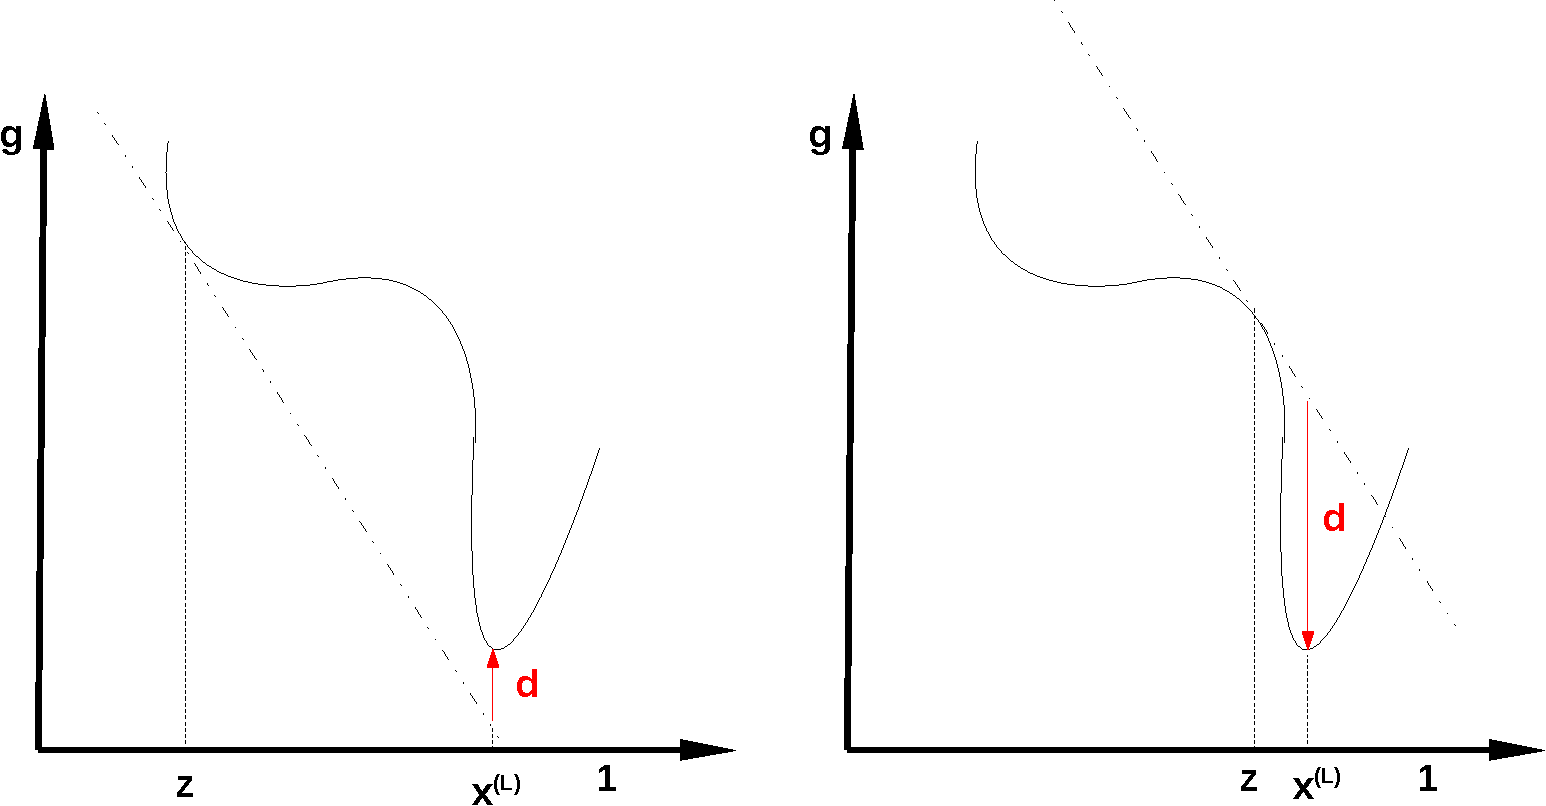
\includegraphics[width=\columnwidth,clip]{./Figs/StabilityCriteria2}\vspace{-0.5cm}
           \caption{Graphical example of two mixtures at different stability condition.} 
        \end{center}
\end{figure}
%%% Figure

\citet{michelsen_1984} used Eqn.~\ref{Chapter:ThermodynamicFormulation:Eqn:Stability_Main} to develop traditional stability tests and the reader should refer to his seminal work. Here \citep[see][]{Henderson_Thesis}, a modified stability test is used that take into account the formulation developed in Sections~\ref{Chapter:ThermodynamicFormulation:Section:MassBalance} and ~\ref{Chapter:ThermodynamicFormulation:Section:GeneralFormulation}.  Replacing $\mfr[x]{i}{L} = 1 - \summation_{i=1}^{n_{c}-1}\mfr[x]{i}{L}$ in the relation $\d=\d\left(\mfr[x]{i}{L}, \cdots, \mfr[x]{n_{c}}{L}\right)$,
\begin{equation}
   \d\left(\mfr[x]{i}{L}, \cdots, \mfr[x]{n_{c}-1}{L}\right) = \summation_{i=1}^{n_{c}-1}\mfr[x]{i}{L}\left[\left(\mfr[\mu]{n_{c}}{V}-\mfr[\mu]{n_{c}}{L}\right)-\left(\mfr[\mu]{i}{V}-\mfr[\mu]{i}{L}\right)\right] - \left(\mfr[\mu]{n_{c}}{V}-\mfr[\mu]{n_{c}}{L}\right).
\end{equation}
From this function we can design an optimisation problem that effectively represents the stability test, Algorithm~\ref{Stability_Test:Algorithm}. This algorithm describes the VLE problem as a function of several intensive properties in the liquid phase.  Thus, during the minimisation algorithm, if the relation $\d\ge 0$ is met then system is assumed stable and there is only one phase, otherwise the mixture is assumed unstable and the system has two phases. 
%%%               %%%
%%%   ALGORITHM   %%%
%%%               %%%
\begin{algorithm}[h]
\begin{shaded}
   \begin{center}
     {\bf Stability Test for the VLE Problem}
   \end{center}

   Given $T$, $P$ and $z_{i}$ $\left(i=1,2,\cdots,n_{c}\right)$. \\
   Find the set of \red{$\mfr[x]{1}{L},\cdots,\mfr[x]{n_{c}-1}{L}$} that \underline{minimises}
   \begin{displaymath}
        \d\left(\mfr[x]{i}{L}, \cdots, \mfr[x]{n_{c}-1}{L}\right) = \summation_{i=1}^{n_{c}-1}\mfr[x]{i}{L}\left[\left(\mfr[\mu]{n_{c}}{V}-\mfr[\mu]{n_{c}}{L}\right)-\left(\mfr[\mu]{i}{V}-\mfr[\mu]{i}{L}\right)\right] - \left(\mfr[\mu]{n_{c}}{V}-\mfr[\mu]{n_{c}}{L}\right)
   \end{displaymath} 
   with $0<\mfr[x]{i}{L}<1,\hspace{.2cm} \forall i=1,\cdots,n_{c}-1$. \\
   Where
   \begin{displaymath}
      \mfr[\mu]{i}{L} = \mfr[\mu]{i}{L} \left(\mfr[x]{1}{L},\cdots,\mfr[x]{n_{c}-1}{L}\right)\text{ and } \mfr[\mu]{i}{V} = \mfr[\mu]{i}{V} \left(z_{1},\cdots, z_{n_{c}}\right)
   \end{displaymath}
\end{shaded}
\label{Stability_Test:Algorithm}\caption{Modified stability test for the VLE problem.}
\end{algorithm}
%%%               %%%
%%%   ALGORITHM   %%%
%%%               %%%

The use of the stability test as it is in Algorithm~\ref{Stability_Test:Algorithm} is convenient to make use of the derived Gibbs-Duhem relations (see Sections~\ref{Chapter:ThermodynamicFormulation:Section:GibbsDuhen}-\ref{Chapter:ThermodynamicFormulation:Section:HessianGibbs}). By differentiating $\d=\d\left(\mfr[x]{i}{L}, \cdots, \mfr[x]{n_{c}-1}{L}\right)$ \wrt $\mfr[x]{j}{k}$ with $j=1,\cdots,n_{c}-1$ and $k=L,V$,
\begin{equation}
   \frc{\partial\d}{\partial\mfr[x]{j}{L}} = \left(\mfr[\mu]{j}{L}-\mfr[\mu]{j}{V}\right) - \left(\mfr[\mu]{n_{c}}{L}-\mfr[\mu]{n_{c}}{V}\right) + \summation_{i=1}^{n_{c}}\mfr[x]{i}{L}\frc{\partial\mfr[\mu]{i}{L}}{\partial\mfr[x]{j}{L}},
\end{equation}
and replacing Eqn.\ref{Chapter:ThermodynamicFormulation:Eqn:GibbsDuhenRelation_2} in Eqn.~\ref{Chapter:ThermodynamicFormulation:Eqn:Stability_Main} results in the elements of the gradient vector of the function $d$ with $j=1,\cdots,n_{c}-1$,
\begin{equation}
   \frc{\partial\d}{\partial\mfr[x]{j}{L}} = \left[\mfr[\mu]{j}{L}\left(\mfr[x]{1}{L},\cdots,\mfr[x]{n_{c}-1}{L}\right) - \mfr[\mu]{j}{V}\left(z_{1},\cdots,z_{n_{c}}\right)\right] - \left[\mfr[\mu]{n_{c}}{L}\left(\mfr[x]{1}{L},\cdots,\mfr[x]{n_{c}-1}{L}\right) \mfr[\mu]{n_{c}}{V}\left(z_{1},\cdots,z_{n_{c}}\right)\right].
\end{equation}
Therefore the Hessian matrix of the function $d$ is,
\begin{equation}
   \frc{\partial^{2}\d}{\partial x_{j}\partial x_{i}} =  \frc{\partial^{2}\d}{\partial x_{i}\partial x_{j}} = \frc{\partial\mfr[\mu]{j}{L}}{\partial\mfr[x]{i}{L}} - \frc{\partial\mfr[\mu]{n_{c}}{L}}{\partial\mfr[x]{i}{L}}, \hspace{.5cm} (i,j)=1,\cdots,n_{c}-1.
\end{equation}

The Hessian matrix is used in the calculation of $\d$ using Newton-based methods as briefly demonstrated in Section~\ref{Chapter:GlobalOpt:Section:NewtonMethods}.
